\section{Methodology}\label{sec:methodology}

\subsection{Dataset}

For practical reasons we decided to use the publically available Face Research Lab London (FRLL) Set~\cite{DeBruine2017}, an ICAO compliant dataset that consists of 102 neutral frontal facial images alongside metadata on attractiveness provided by over 2500 observers. We carefully selected 15 demographically diverse facial
images out of the dataset, shown in Fig.~\ref{fig:subdataset}. Each image was subsequently processed using four printer-proof steganography methods, each applied at nine encoding threshold levels. This approach introduced a diverse range of quality distortions, yielding a total of 555 images, including their original references.

\begin{figure}[!htbp]
    \centering
    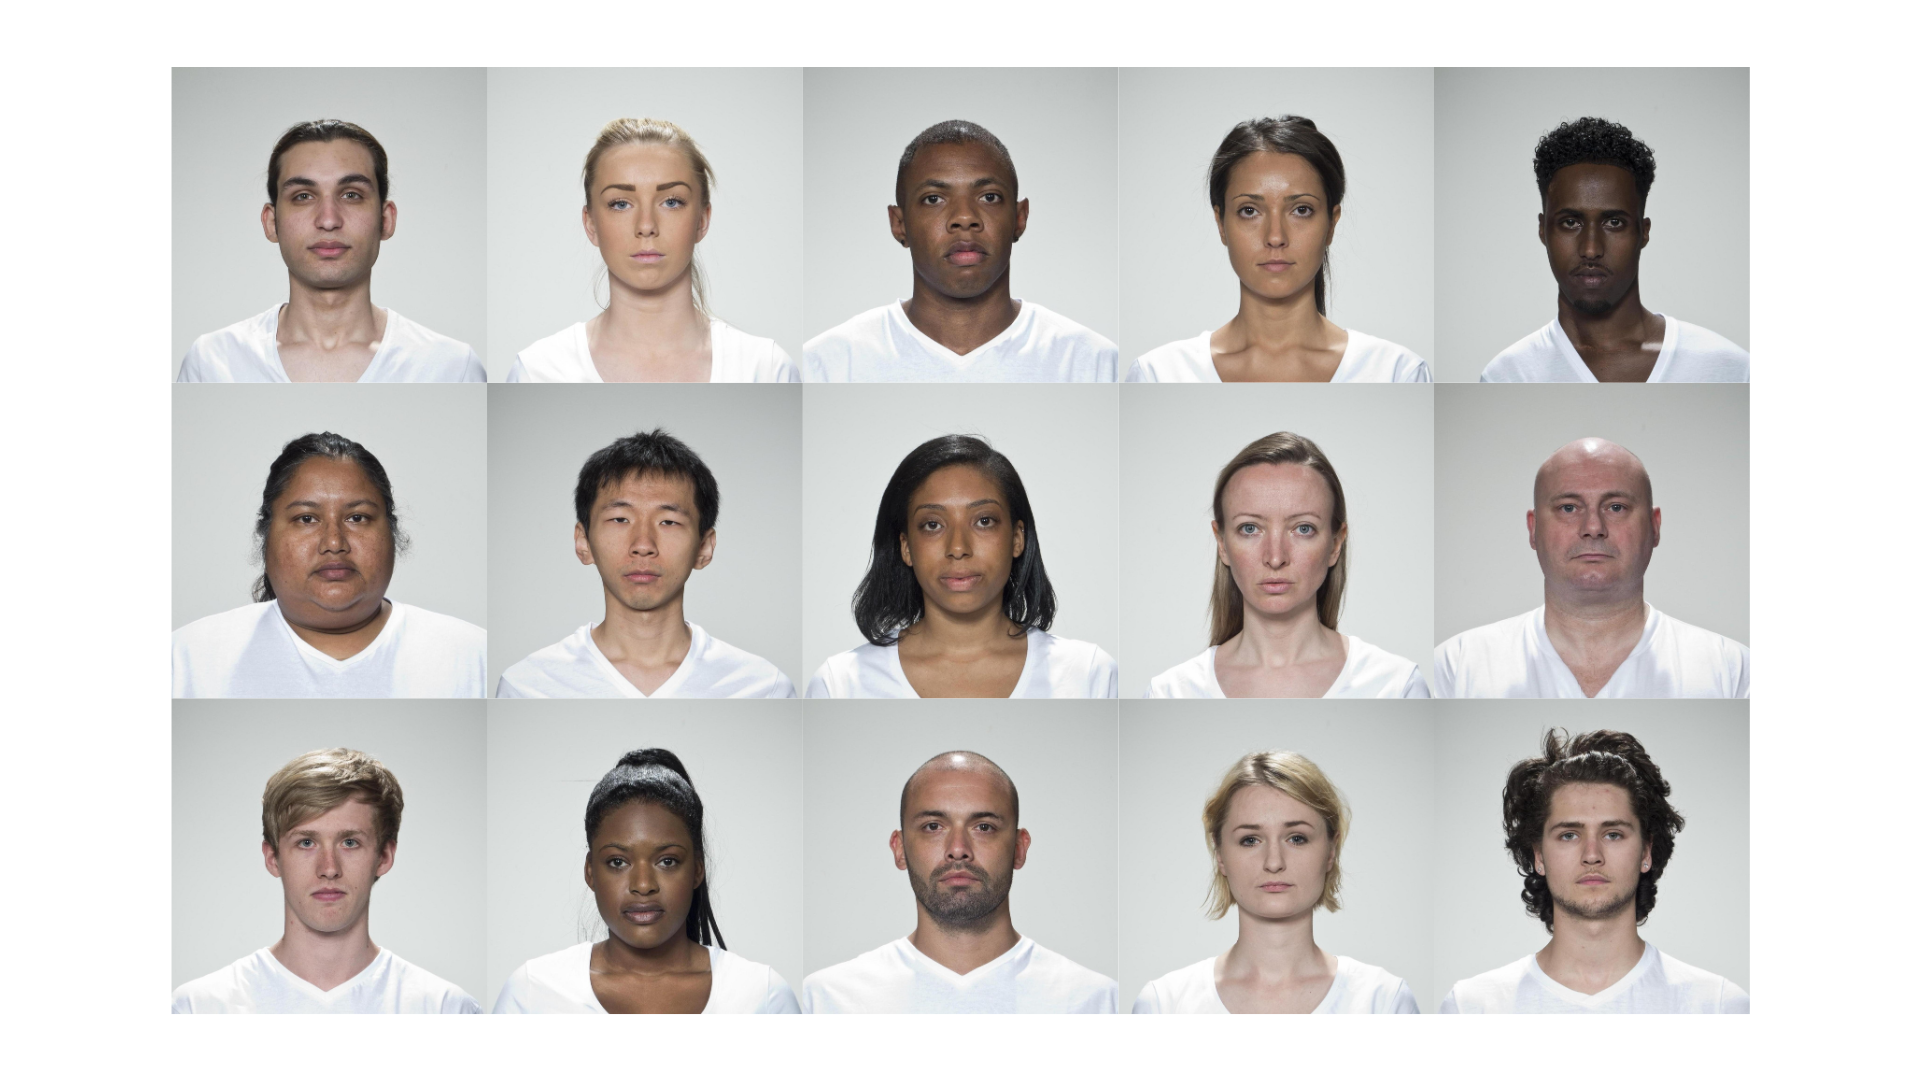
\includegraphics[width=1\linewidth]{images/subdataset.png}
    \caption{Sample images from the FRLL dataset.}\label{fig:subdataset}
\end{figure}

The used printer-proof steganography methods are based on Generative Adversarial Networks (GANs)~\cite{gans2018} to encode and decode information, we can obtain various results depending on the method used:

\begin{itemize}
    \item StegaStamp~\cite{stegastamp2020}: claims to be the first steganography model capable of decoding data from printed images. The authors show robust results in decoding data under physical transmission by developing novel strategies to add noise in the training process, printer noise simulation, and distortion for the training dataset.
    \item CodeFace~\cite{codeface2021}: encoder and decoder networks are trained using end-to-end GANs. It introduces a new security system for encoding and decoding facial images that are printed in common IDs and MRTDs.
    \item RiemStega~\cite{cruz2025riemstega}: proposes a new loss function that extends the loss function based on the $L_2$ distance between images to the Riemannian manifold of symmetric and positive definite matrices.
    \item StampOne~\cite{stampone2023}: focuses on high-level robust steganography, such as~\cite{codeface2021, stegastamp2020}, striking a balance between high-quality encoded images and decoding accuracy. It mitigates distortion-related issues like JPEG compression, camera sensors and printer's Gaussian noise by incorporating gradient transform, wavelet transform, and Depthwise~\cite{tay2022efficient} to normalize and balance frequencies of the inputs. 
\end{itemize}

Each image in our dataset was evaluated approximately 30 times by human observers, providing a robust Mean Opinion Score (MOS) dataset.

We followed ITU-R BT.500 --- 15~\cite{ITU-R-BT500} recommendation, and adopted the Single Stimulus method. Around 200 different observers were carefully instructed on how to perform the test session, the average duration of the session was 22 minutes, and the average number of tests in each session was 70. Resulting in over 14,000 images being evaluated.

To conduct the sessions we created a webapp, seen in Fig.~\ref{fig:platform}, where the observers conceded their demographic data (age, gender, ethnicity, etc.) and were asked to evaluate each image on a scale from 1 to 100 using a slider bar, for as long as they wanted. The rating scale was divided into five categorical levels: scores from 1 to 25 were classified as Bad, 26 to 50 as Poor, 51 to 75 as Fair, 76 to 99 as Good, and a score of 100 as Excellent.

\begin{figure}[!htbp]
    \centering
    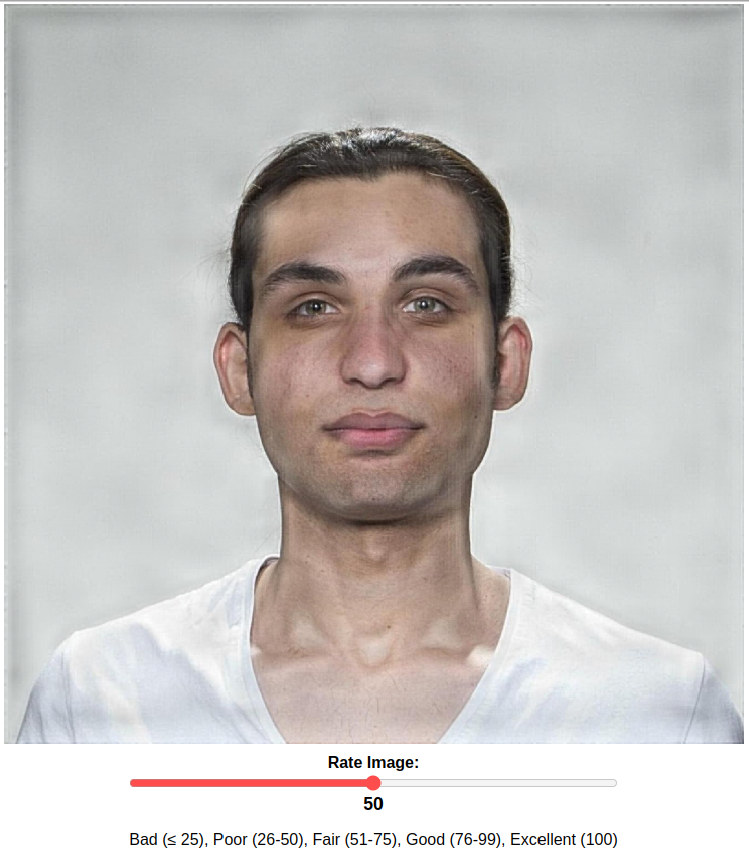
\includegraphics[width=0.7\linewidth]{images/webapp.png}
    \caption{Custom webapp platform used to access overall image quality.}\label{fig:platform}
\end{figure}

We collected observer's demographic (age, gender, ethnicity, and country of origin) and non-demographic information (education level, device being used, and place where test was being performed).

\subsection{Statistical Bias Analysis}

Considering that the homogeneity of variances assumption is not met, we performed Welch's analysis of variance (ANOVA) to examine the impact of observer demographics --- gender (140 male, 60 female), ethnicity (173 causasian, 8 latino, 8 black, and others), and age grouped into categories (under 18, 18 --- 25, 26 --- 40, 41 --- 60, over 60) as well as subject demographic and non-demographic (attractiveness) characteristics on MOS.\@ The statistical significance of each factor was evaluated using a threshold of $p < 0.01$, and effect size analysis was conducted using Eta Squared~\cite{cohen1988statistical} ($\eta^2$) to quantify the relative contribution of each variable.

\subsubsection{Impact of Observer Demographics on MOS}

According to table~\ref{tab:anova_observer}, ethnicity, gender and age significantly impact MOS scores, suggesting that subjective evaluations of image quality are influenced by observer characteristics. Post-hoc Tukey's HSD~\cite{tukey1949comparing} tests were conducted to determine specific group differences, identifying notable discrepancies across demographic subgroups. The presence of these biases underscores the need for IQA methodologies that incorporate perceptual fairness considerations.


\begin{table}[!htbp]
\caption{Welch's ANOVA results for observer demographics.}
\begin{center}
\begin{tabular}{|l|c|c|c|c|}
\hline
\textbf{Factor} & \textbf{Welch F} & \textbf{DF} & \textbf{p-value} & \textbf{Eta Squared}  \\
\hline
Observer Gender & 6.97 & 1 & 0.00112 & 0.012 \\ \hline
Observer Ethnicity & 9.36 & 8 & 5.65e-13 & 0.027 \\ \hline
Observer Age Group & 33.00 & 4 & $\cong$ 0 & 0.045 \\ \hline
\end{tabular}\label{tab:anova_observer}
\end{center}
\end{table}

\subsubsection{Impact of Image Characteristics on MOS}

Table~\ref{tab:anova_image} presents the influence of subject demographic and non-demographic characteristics on MOS.\@ Results suggest that MOS is influenced by aesthetic preferences and other visual factors, reinforcing its inherently subjective nature.

\begin{table}[!htbp]
\caption{Welch's ANOVA results for subject characteristics.}
\begin{center}
\begin{tabular}{|l|c|c|c|c|}
\hline
\textbf{Factor} & \textbf{Welch F} & \textbf{DF} & \textbf{p-value} & \textbf{Eta Squared} \\
\hline
Subject Gender & 19.84 & 1 & 5.87e-06 & 0.018 \\
\hline
Subject Ethnicity & 8.85 & 3 & 7.38e-06 & 0.022 \\
\hline
Subject Age Group & 11.62 & 4 & 4.82e-35 & 0.033 \\
\hline
Attractiveness & 18.04 & 1 & 2.18e-05 & 0.015 \\
\hline
\end{tabular}\label{tab:anova_image}
\end{center}
\end{table}

\subsubsection{Observer-Subject Interaction Effects on MOS}

A two-way ANOVA was performed to analyze the interaction effects between observer demographics and subject characteristics.

\begin{table}[!htbp]
\centering
\caption{Two-way ANOVA interaction effects.}
\begin{tabular}{|l|c|c|c|c|} \hline
\textbf{Observer $\times$ Subject} & \textbf{F-value} & \textbf{DF} & \textbf{p-value} & \textbf{Eta Squared} \\ \hline
Gender & 2.31 & 1 & 0.0654 & 0.006 \\ \hline
Ethnicity & 1.51 & 24 & 0.0556 & 0.011 \\ \hline
Age Group & 2.87 & 16 & 1.94e-10 & 0.024 \\ \hline
\end{tabular}\label{tab:anova_interaction}
\end{table}

These findings confirm the existence of demographic bias in MOS ratings, making it crucial to account for such biases when using subjective scores in image quality assessment models. The effect size analysis using Eta Squared ($\eta^2$) provides insight into the relative contribution of each factor to MOS variance. Our results reinforce the need for better FIQA models to correct demographic biases.

\subsection{Image Quality Metrics}

A total of 41 different Image Quality Assessment (IQA) metrics were evaluated, spanning traditional signal-based measures (e.g., PSNR, SSIM), perceptual-based metrics (e.g., FSIM, VIF), and deep-learning-based approaches (e.g., LPIPS, DISTS). The correlation between these metrics and MOS was analyzed using Pearson’s and Spearman’s correlation coefficients. 

Fig.~\ref{fig:mos_vs_iqa} presents scatter plots comparing MOS values against individual IQA metrics. Each plot illustrates the relationship between subjective evaluations and objective IQA scores, highlighting the varying degrees of correlation among metrics. Some metrics, such as FSIM and MS-SSIM~\cite{wang2003multiscale}, demonstrate a strong monotonic relationship with MOS.\@ These visualizations justify the need for a fusion-based approach to optimize MOS predictability.


\begin{figure}[h]
    \centering
    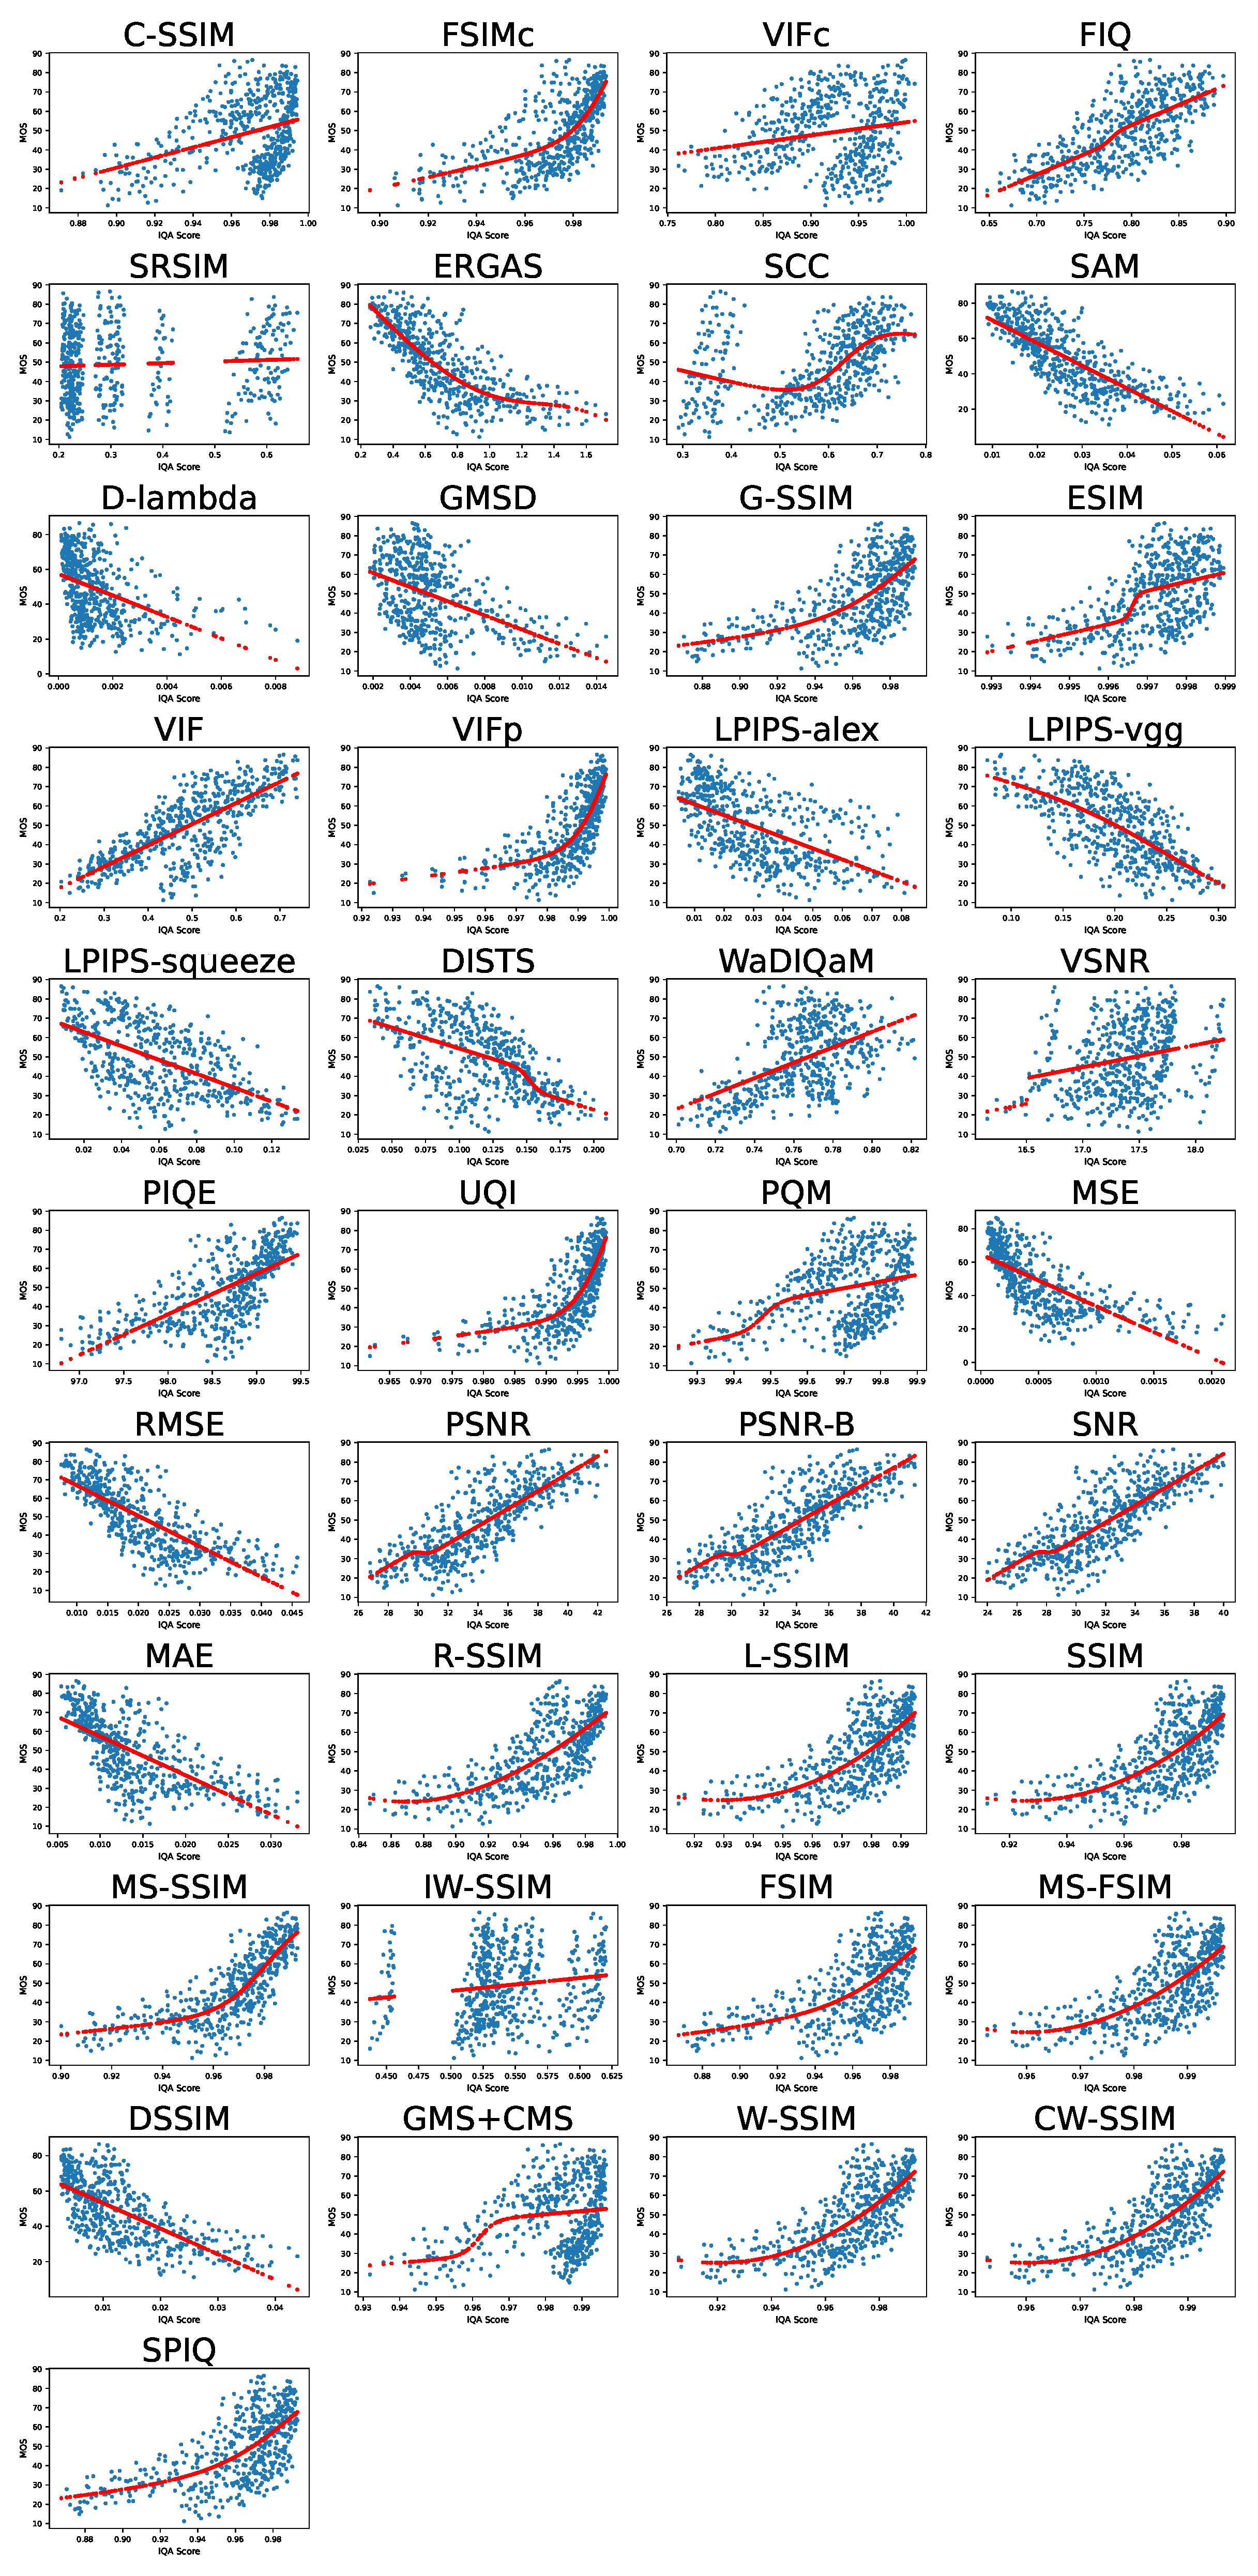
\includegraphics[width=\linewidth]{images/mos_vs_iqa_grid.eps}
    \caption{Scatter plots illustrating the relationship between Mean Opinion Scores (MOS) and individual Image Quality Assessment (IQA) metrics.}\label{fig:mos_vs_iqa}
\end{figure}

\subsection{Fusion-Based Image Quality Assessment}

To improve the correlation between IQA metrics and MOS, we implemented a fusion-based approach integrating multiple quality measures. The fusion process involved weighting individual IQA metrics based on their predictive performance relative to MOS.\@ We explored several fusion techniques, including:

\begin{itemize}
    \item Principal Component Analysis (PCA): Used to reduce redundancy among IQA metrics and derive an optimized linear combination.
    \item Regression-Based Models: Linear regression and ridge regression were applied to determine the best combination of metrics that predict MOS effectively.
    \item Machine Learning Approaches: A Random Forest~\cite{breiman2001random} (RF) model was trained using individual IQA metrics as input features, leveraging nonlinear interactions to improve MOS correlation. The dataset was split into 80\% for training and 20\% for testing. The model was configured with 100 trees (\textit{n\_estimators = 100}) and used the MSE criterion for optimization.

\end{itemize}

To assess the effectiveness of individual and fusion-based IQA metrics, we employed two correlation measures:

\begin{itemize}
    \item Pearson's Linear Correlation Coefficient (PLCC): Evaluates the linear relationship between IQA scores and MOS.\@
    \item Spearman's Rank-Order Correlation Coefficient (SRCC): Measures the monotonic relationship between IQA scores and MOS, accounting for nonlinearity in observer perception.
\end{itemize}

\subsection{Implementation Details}

The experiments were conducted using Python. The dataset went through a post-screening process to normalize IQA scores and eliminate outliers. Training and evaluation followed a five-fold cross-validation strategy to ensure robust model performance.
